
%(BEGIN_QUESTION)
% Copyright 2006, Tony R. Kuphaldt, released under the Creative Commons Attribution License (v 1.0)
% This means you may do almost anything with this work of mine, so long as you give me proper credit

En væske strømmer inn i en lagringstank:

$$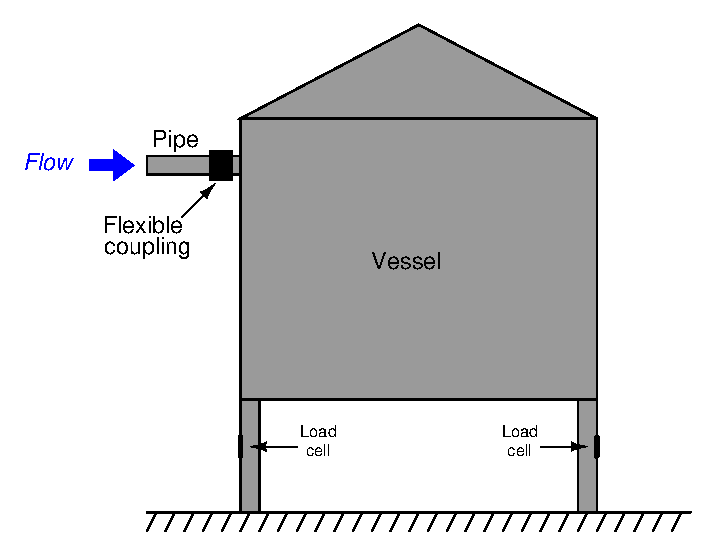
\includegraphics[width=15.5cm]{i01552x01.eps}$$

Lastceller montert på tankens støttebein gir en måte å måle akkumulert væskemasse på. En datamaskin logger tankens bruttovekt med 5 minutters intervaller:

% No blank lines allowed between lines of an \halign structure!
% I use comments (%) instead, so that TeX doesn't choke.

$$\vbox{\offinterlineskip
\halign{\strut
\vrule \quad\hfil # \ \hfil & 
\vrule \quad\hfil # \ \hfil \vrule \cr
\noalign{\hrule}
%
% First row
Bruttovekt & Tid \cr
%
(pund) & (time:minutt) \cr
%
\noalign{\hrule}
%
% Another row
1342 & 4:55 \cr
%
\noalign{\hrule}
%
% Another row
2003 & 5:00 \cr
%
\noalign{\hrule}
%
% Another row
2624 & 5:05 \cr
%
\noalign{\hrule}
%
% Another row
3255 & 5:10 \cr
%
\noalign{\hrule}
%
% Another row
3927 & 5:15 \cr
%
\noalign{\hrule}
} % End of \halign 
}$$ % End of \vbox

Beregn følgende:

\begin{itemize}
\item{} Massestrømningsraten til væsken (i enheter pund per time) ved 5:07
\vskip 10pt
\item{} Gjennomsnittlig massestrømningsrate for væsken (i enheter pund per time) siden begynnelsen av timen
\end{itemize}

\vskip 10pt

\vfil 

\underbar{file i01552}
\eject
%(END_QUESTION)





%(BEGIN_ANSWER)

Dette er et vurdert spørsmål -- ingen svar eller hint gitt!

%(END_ANSWER)





%(BEGIN_NOTES)

Massestrømningsraten ved 5:07 estimeres best ved å beregne en differansekvotient mellom 5:05 og 5:10:

$$\overline{W} = {\Delta m \over \Delta t} = {3255 \hbox{ lb} - 2624 \hbox{ lb} \over 5:10 - 5:05} = {631 \hbox{ lb} \over 5 \hbox{ min}} = {631 \hbox{ lb} \over 0.0833 \hbox{ hr}} = 7572 \hbox{ lb/hr}$$

\vskip 10pt

Gjennomsnittlig massestrømningsrate siden starten av timen estimeres best ved å beregne en differansekvotient mellom 5:00 og 5:15:

$$\overline{W} = {\Delta m \over \Delta t} = {3927 \hbox{ lb} - 2003 \hbox{ lb} \over 5:15 - 5:00} = {1924 \hbox{ lb} \over 15 \hbox{ min}} = {1924 \hbox{ lb} \over 0.25 \hbox{ hr}} = 7696 \hbox{ lb/hr}$$

\vskip 10pt

Hvis man ikke leser spørsmålet nøye, kan man feilaktig beregne gjennomsnittlig massestrømningsrate for hele perioden dokumentert i tabellen. Dette er resultatet:

$$\overline{W} = {\Delta m \over \Delta t} = {3927 \hbox{ lb} - 1342 \hbox{ lb} \over 5:15 - 4:55} = {2585 \hbox{ lb} \over 20 \hbox{ min}} = {2585 \hbox{ lb} \over 0.3333 \hbox{ hr}} = 7755 \hbox{ lb/hr}$$

%INDEX% Mathematics, calculus: derivative (calculating flow rates from measured volumes at specific times)

%(END_NOTES)

